\chapter{Realisierung}
\label{ch:Realisierung}
% TODO Beschreibung der Umsetzung der definierten Ziele, einschliesslich der aufgetretenen Schwierigkeiten und Einschränkungen
In diesem Kapitel wird die ganze Realisierung des Projektes beschrieben, einschliesslich der aufgetretenen
Schwierigkeiten und Einschränkungen. Dabei geht es darum, die Umsetzung der definierten Ziele aufzuzeigen.

\section{Aufbau Datensatz}
\label{sec:aufbau_datensatz}
Wie in Kaptiel \fullref{sec:abschliessende_problemdefinition} beschrieben, wird ein Datensatz mit Texten aufgebaut,
welchem dem Label $ erwachsen $, sowie dem Label $ kindlich $ zugeteilt werden können. Die Quellen der Texte sind Online
Lexikas. Wikipedia dient dabei als Quelle für Sätze des Labels $ erwachsen $, analog dient das Klexikon als Quelle für
Sätze des Labels $ kindlich $. Für das Zusammentragen der Texte wurde ein Crawler realisiert, welcher die Artikel aus
dem Klexikon und Wikipedia zusammenträgt.

\subsection{Reinigung des Datensatz}
\label{sub:reinigung_des_datensatz}
Die Artikel wurden entsprechend gereinigt und die einzelnen Sätze aus den Artikeln extrahiert. Dabei wurde auf das
Framework Natural Language Toolkit (NLTK) zurückgegriffen. Die Pipeline für die Reinigung und der Extrahierung wurde
dabei wie folgt aufgebaut.
\newline
\begin{enumerate}
	\setlength\itemsep{0em}
	\item Reinigung der Strings durch ersetzen von Buchstaben mit Akzent zeichen wie z.B. è, à, â, ê.
	\item Einheitliche Verwendung von Anführszeichen.
	\item Einfügen von Leerschläge bei Kommas (,), Gedankenstichen (-), Schrägstrichen (/), Doppelpunkt (:), Strichpunkt
	(;) sowie an Satzenden.
	\item Tokenizierung der Arikel zu Sätzen mithilfe von NLTK. Dabei wurden nur Sätze erlaubt, welche gewisse Charaktere
	enthalten.
	\item Anpassung der Grossschreibung der Satzanfänge mithilfe von TreeTagger. Dabei wurde die Grossschreibung nur beibehalten, falls das Wort
    ein Nomen oder Eigennamen ist.
\end{enumerate}
\noindent
Weiter wurden Daten für die statistische Analyse der Datenquelle sowie der Sätze mitaufgezeichned. Dies, um in einem
nächsten Schritt, den Datensatz weiter zu bereiningen. Für die Datenquellen wurden folgende Daten aufgezeichnet.
\begin{enumerate}
    \setlength\itemsep{0em}
    \item Anzahl an Artikel aus der Datenquelle
    \item Anzahl Sätze aus der Datenquelle
    \item Anzahl Wörter aus der Datenquelle
\end{enumerate}
\noindent
Für die Analyse der einzelnen Sätze wurde während der Reinigung der Sätze folgendes mitabgespeichert.
\begin{enumerate}
    \setlength\itemsep{0em}
    \item Datenquelle des Satzes
    \item Artikel des Satzes
    \item Anzahl Wörter im Satz
\end{enumerate}
\noindent
So entstand aus den Artikeln der einzelnen Datenquelle ein gemeinsamer Datensatz, abgespeichert als CSV, welcher
folgende Struktur aufweist.
\begin{verbatim}
source	article	length	sentence
klexikon	Aal	9	Aale sind Fische , die wie Schlangen aussehen .
klexikon	Aal	10	ihre Körper sind sehr lang , schlank und beweglich .
klexikon	Aal	13	sie haben eher kleine Flossen , die wie Bänder am Körper anliegen .
wikipedia	Reh	7	die Fluchtdistanz von Feldrehen ist hoch .
wikipedia	Reh	8	diese hohe Fluchtdistanz kompensiert die fehlende Deckung .
\end{verbatim}

\subsection{Statistische Analyse des Datensatz}
\label{sub:statistische_analyse_des_datensatz}
In einem weiteren Schritt wurde der Datensatz statistisch analysiert. Dies, um den Datensatz weiter zu reinigen und zu
normalisieren. Dabei soll zuerst die Zählung der Artikel, Sätze, sowie der Wörter aufgezeigt werden.
\begin{figure}[H]
    \minipage{0.32\textwidth}
      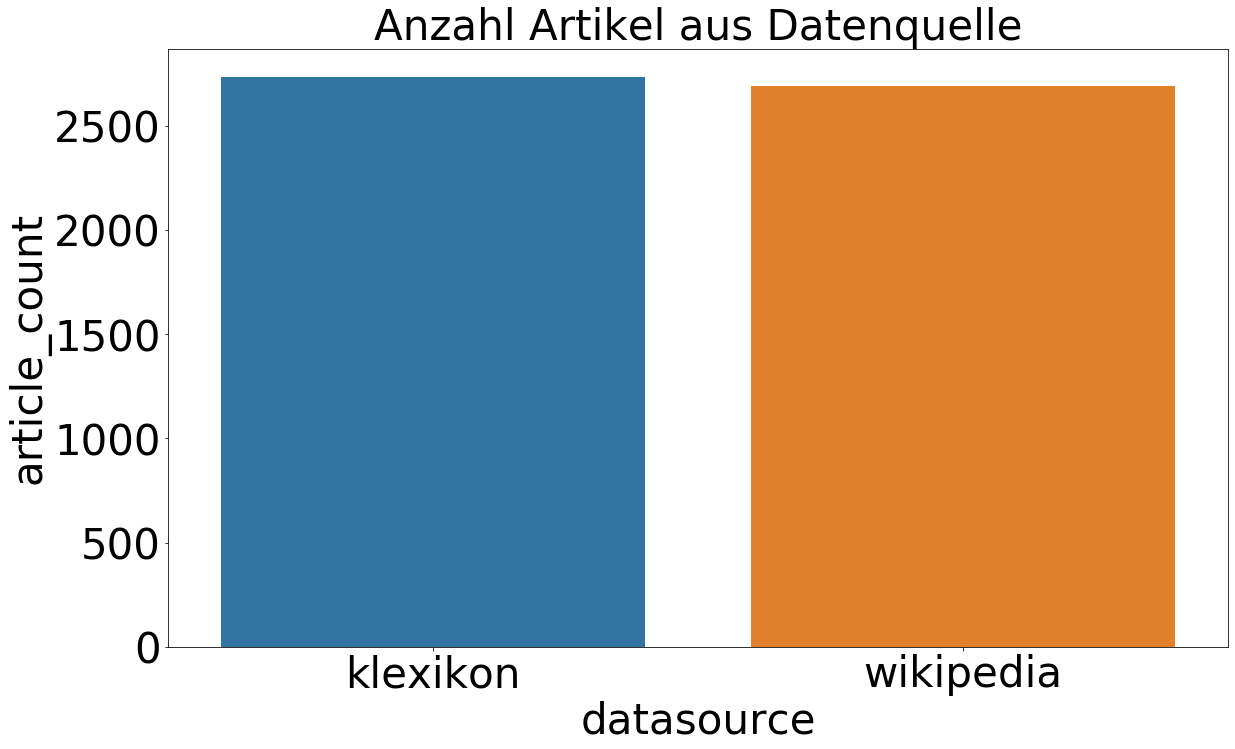
\includegraphics[width=\linewidth]{article_count_ds.png}
      \caption{Anz. Artikel im Datensatz}\label{fig:article_count_ds}
    \endminipage\hfill
    \minipage{0.32\textwidth}
      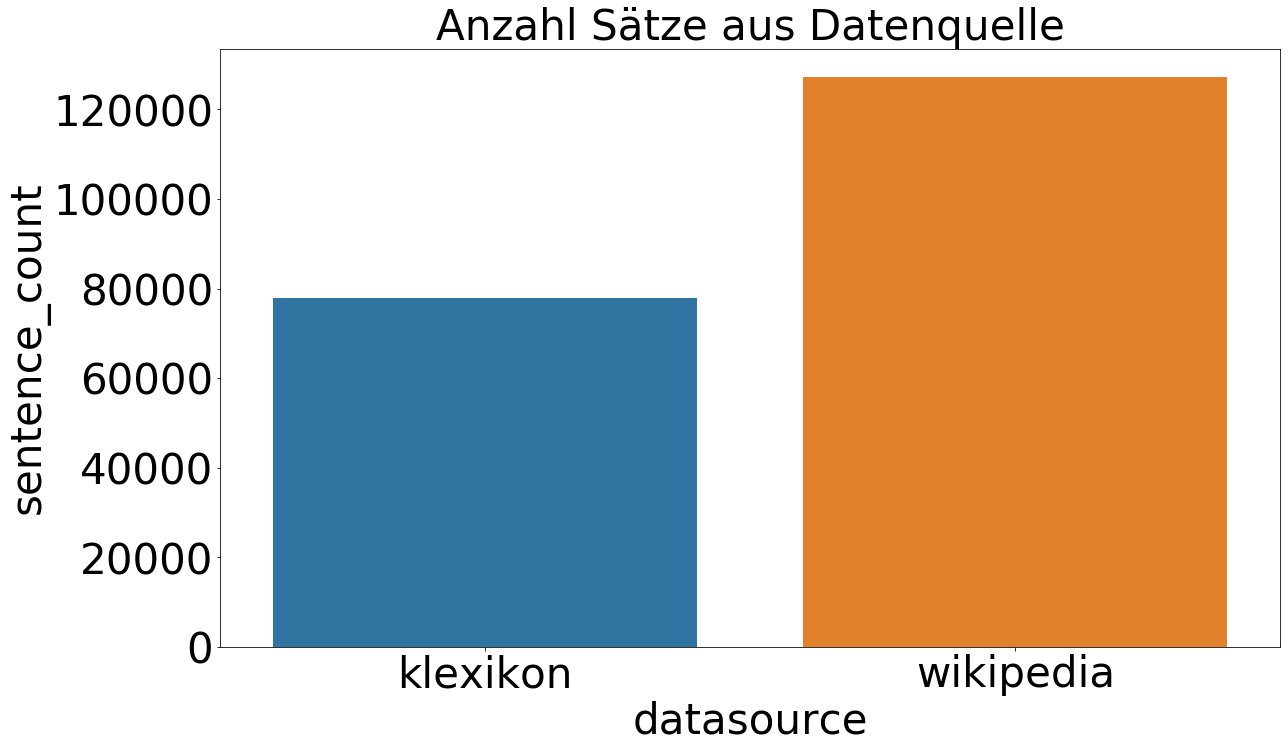
\includegraphics[width=\linewidth]{sentence_count_ds.png}
      \caption{Anz. Sätze im Datensatz}\label{fig:sentence_count_ds}
    \endminipage\hfill
    \minipage{0.32\textwidth}
      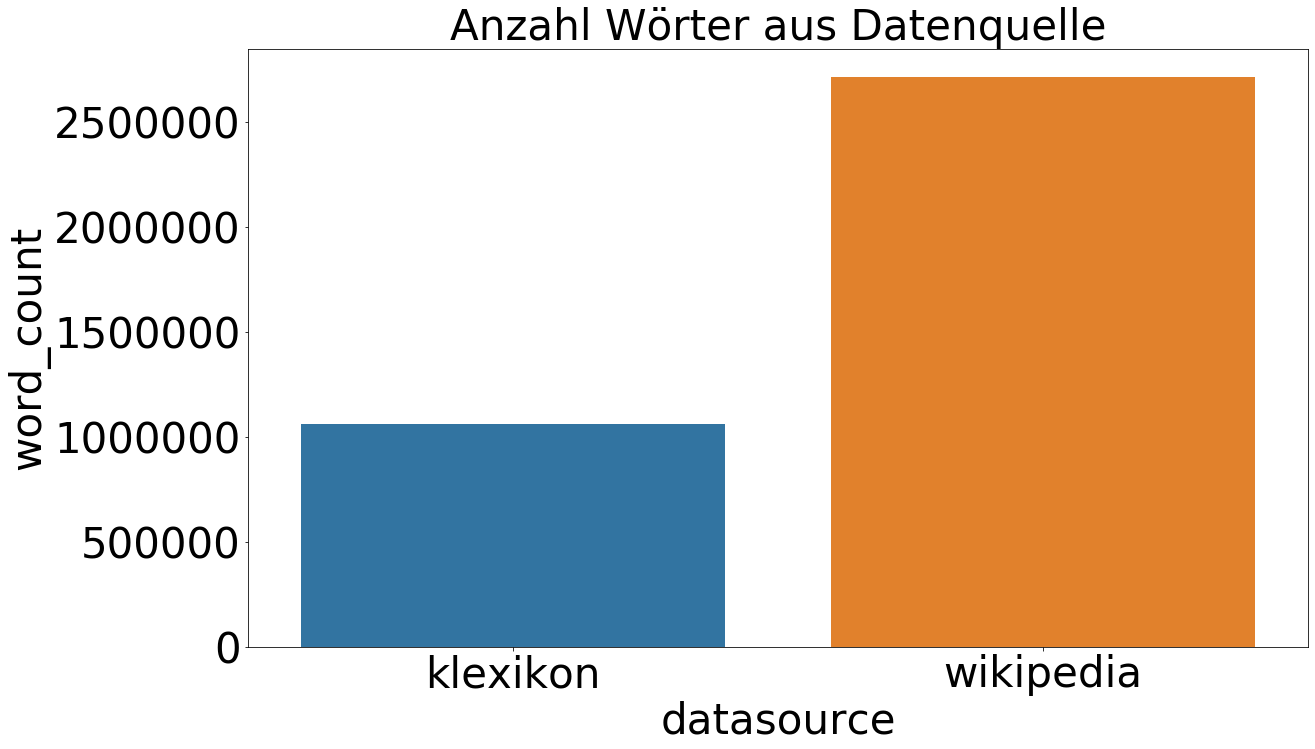
\includegraphics[width=\linewidth]{word_count_ds.png}
      \caption{Anz. Wörter im Datensatz}\label{fig:word_count_ds}
    \endminipage       
\end{figure}
\begin{table}[H]
  \centering
  \begin{tabular}{|c|c|c|c|}
      \hline
      \textbf{Datenquelle}& \textbf{Anz. Artikel}& \textbf{Anz. Sätze}& \textbf{Anz. Wörter}\\
      \hline
      \textbf{Klexikon}& 2'733 & 77'924 & 1'058'623\\
      \hline
      \textbf{Wikipedia}& 2'689 & 127'177 & 2'710'452\\
      \hline
  \end{tabular}
  \caption{Anzahl der Artikel, Sätze und Wörter aus Wikipedia und Klexikon.}
\label{tab:dataset_count_wiki_klexi_base}
\end{table}
\noindent
Wie angenommen sind die Artikel von Wikipedia umfangreicher als die vom Klexikon. Die Artikel beinhalten mehr Sätze als
aus dem Lexikon. Entsprechend auch mehr Wörter. Dies kann auch anhand der Verteilung für Sätze pro Artikel aufgezeigt
werden, siehe \ref{fig:distribution_sentence_klexi} und \ref{fig:distribution_sentence_wiki}.
\begin{figure}[H]
  \minipage{0.45\textwidth}
    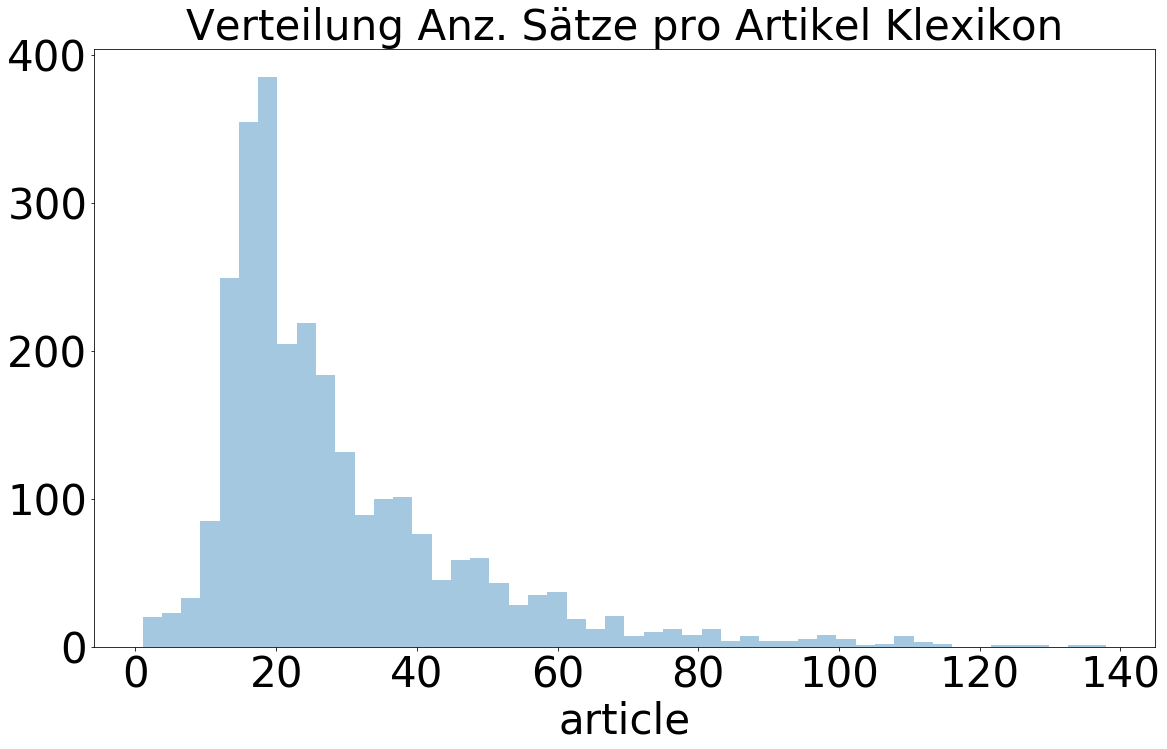
\includegraphics[width=\linewidth]{distribution_sentence_klexi.png}
    \caption{Verteilung Sätze pro Artikel Klexikon}\label{fig:distribution_sentence_klexi}
  \endminipage\hfill
  \minipage{0.45\textwidth}
    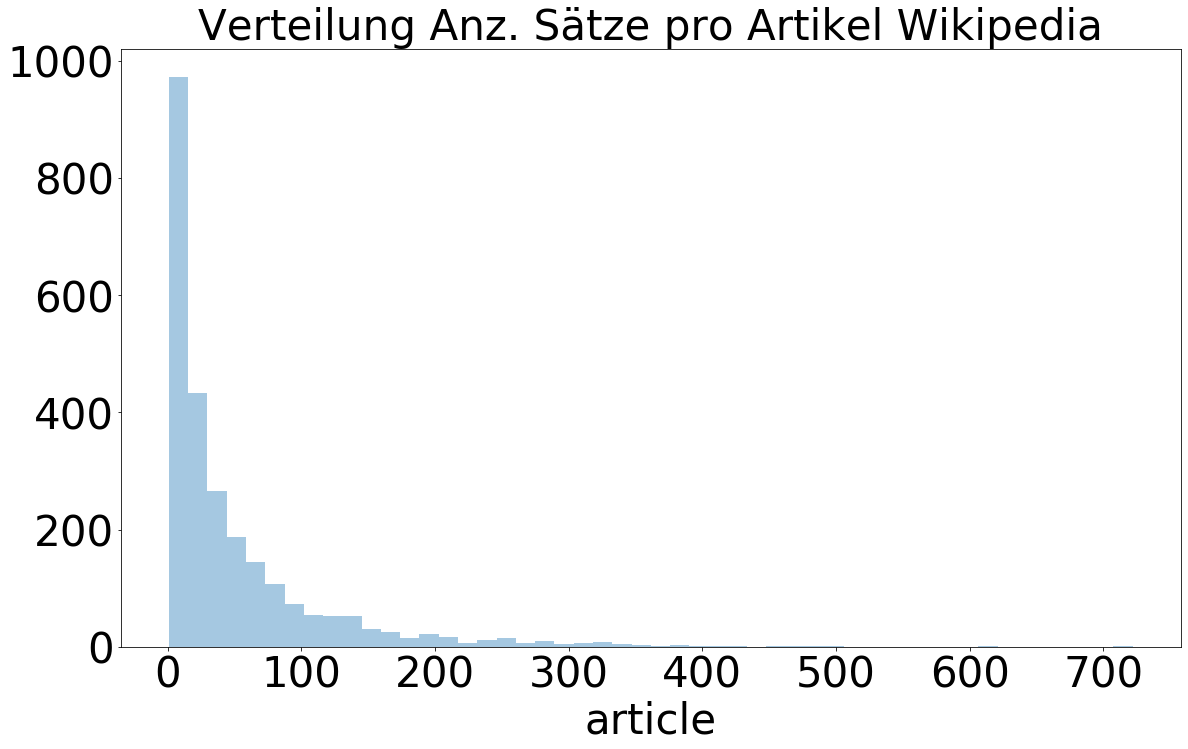
\includegraphics[width=\linewidth]{distribution_sentence_wiki.png}
    \caption{Verteilung Sätze pro Artikel Wikipedia}\label{fig:distribution_sentence_wiki}
  \endminipage\hfill     
\end{figure}
\begin{table}[H]
  \centering
  \begin{tabular}{|c|c|c|c|c|c|}
      \hline
      \textbf{Datenquelle}& \textbf{25\% Quartil}& \textbf{Median}& \textbf{75\% Quartil} & \textbf{Mean} &
      \textbf{Standardabweichung}\\
      \hline
      \textbf{Klexikon}& 17 & 23 & 35 & 28.6 & 18.3\\
      \hline
      \textbf{Wikipedia}& 8 & 24 & 63 & 49.9 & 70.0\\
      \hline
  \end{tabular}
  \caption{Verteilung der Anzahl Sätze pro Artikel für Klexikon und Wikipedia}
\label{tab:distribution_sentences_per_article}
\end{table}
\noindent
Für die Problemstellung ist jedoch die Verteilung der Anzahl Wörter in einem Satz relevant. Daher wurden Sätze mit
weniger als $ 4 $ Wörter aus dem Datensatz entfernt. Dies, da Sätze mit $ 3 $ oder weniger Wörter eine zu geringe
Relevanz für diverse Stile aufweisen. Anhand der Grafiken \ref{fig:distribution_klexi_unclean} und
\ref{fig:distribution_wiki_unclean} wird gezeigt, dass die Sätze aus Wikipedia länger gestaltet sind als die Sätze aus
dem Klexikon. Hier wird auch wie in \fullref{sec:abschliessende_problemdefinition} beschrieben, das Ziel des Style
Transfer legitimiert.
\begin{figure}[H]
  \minipage{0.45\textwidth}
    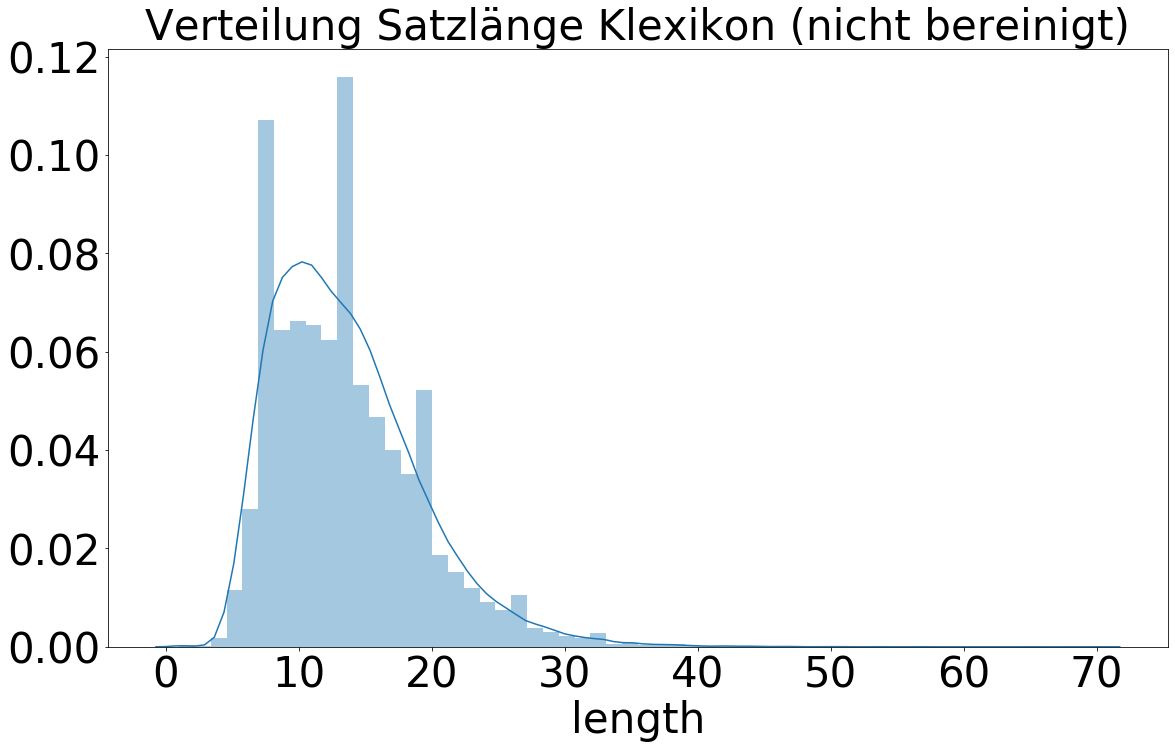
\includegraphics[width=\linewidth]{distribution_klexi_unclean.png}
    \caption{Verteilung Satzlänge Klexikon nicht bereinigt}\label{fig:distribution_klexi_unclean}
  \endminipage\hfill
  \minipage{0.45\textwidth}
    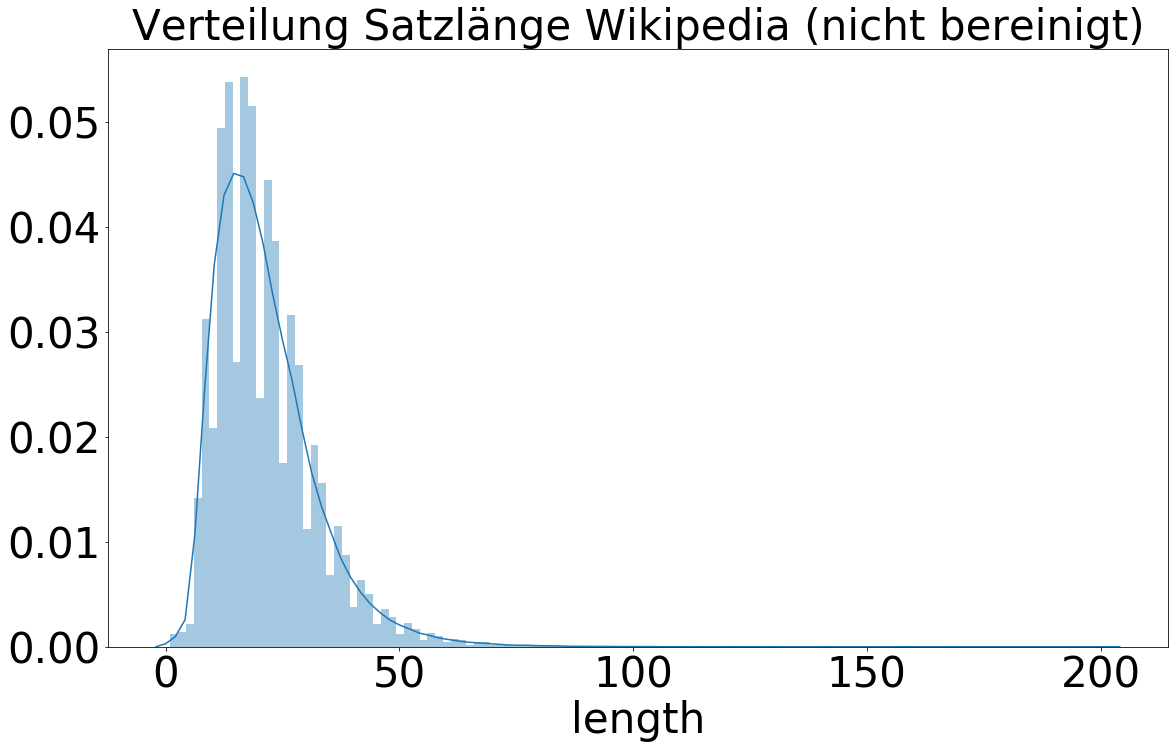
\includegraphics[width=\linewidth]{distribution_wiki_unclean.png}
    \caption{Verteilung Satzlänge Wikipedia nicht bereinigt}\label{fig:distribution_wiki_unclean}
  \endminipage\hfill     
\end{figure}
\begin{table}[H]
  \centering
  \begin{tabular}{|c|c|c|c|c|c|}
    \hline
    \textbf{Datenquelle}& \textbf{25\% Quartil}& \textbf{Median}& \textbf{75\% Quartil} & \textbf{Mean} &
    \textbf{Standardabweichung}\\
    \hline
    \textbf{Klexikon}& 9 & 13 & 17 & 13.6 & 5.5\\
    \hline
    \textbf{Wikipedia}& 14 & 19 & 27 & 21.4 & 10.8\\
    \hline
  \end{tabular}
  \caption{Verteilung Anzahl Wörter Klexikon und Wikipedia}
\label{tab:distribution_klexi_wiki_unclean}
\end{table}
\noindent
Mit Hilfe des \gls{IQR} wurden die Ausreisser aus dem Datensatz entfernt. Dabei gibt es nur Aussreisser im oberen
Bereich, da die untere Grenze unter $ 0 $ liegt. Mit der Entferung der zu kurzen Sätze, unter $ 4 $ Wörter, und Sätze
über dem oberen \gls{IQR} repräsentiert der Datenstatz weiterhin das Ziel der \fullref{sec:Problemdefinition}. Dieser
Datenbestand bildet die Basis für weitere Datensätze, siehe \fullref{sub:datensatz_ausgeglichen} und
\fullref{sub:datensatz_gekuertz}.
\begin{figure}[H]
  \minipage{0.45\textwidth}
    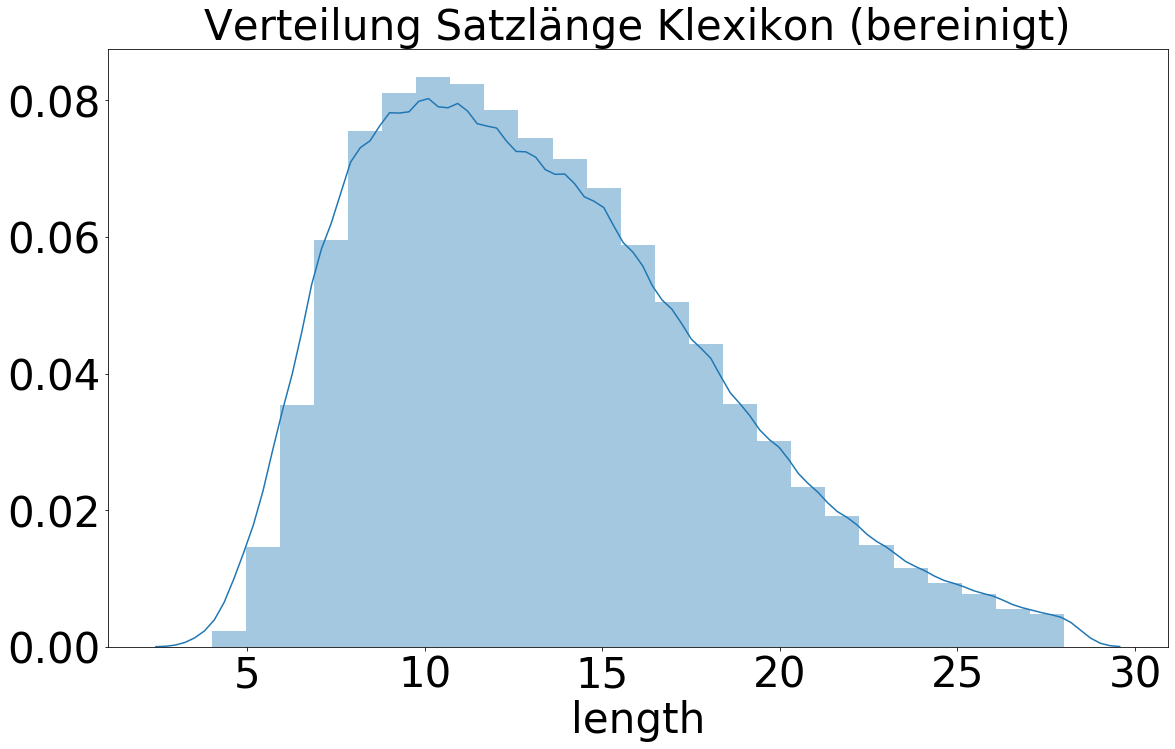
\includegraphics[width=\linewidth]{distribution_klexi_clean.png}
    \caption{Verteilung Satzlänge Klexikon bereinigt}\label{fig:distribution_klexi_clean}
  \endminipage\hfill
  \minipage{0.45\textwidth}
    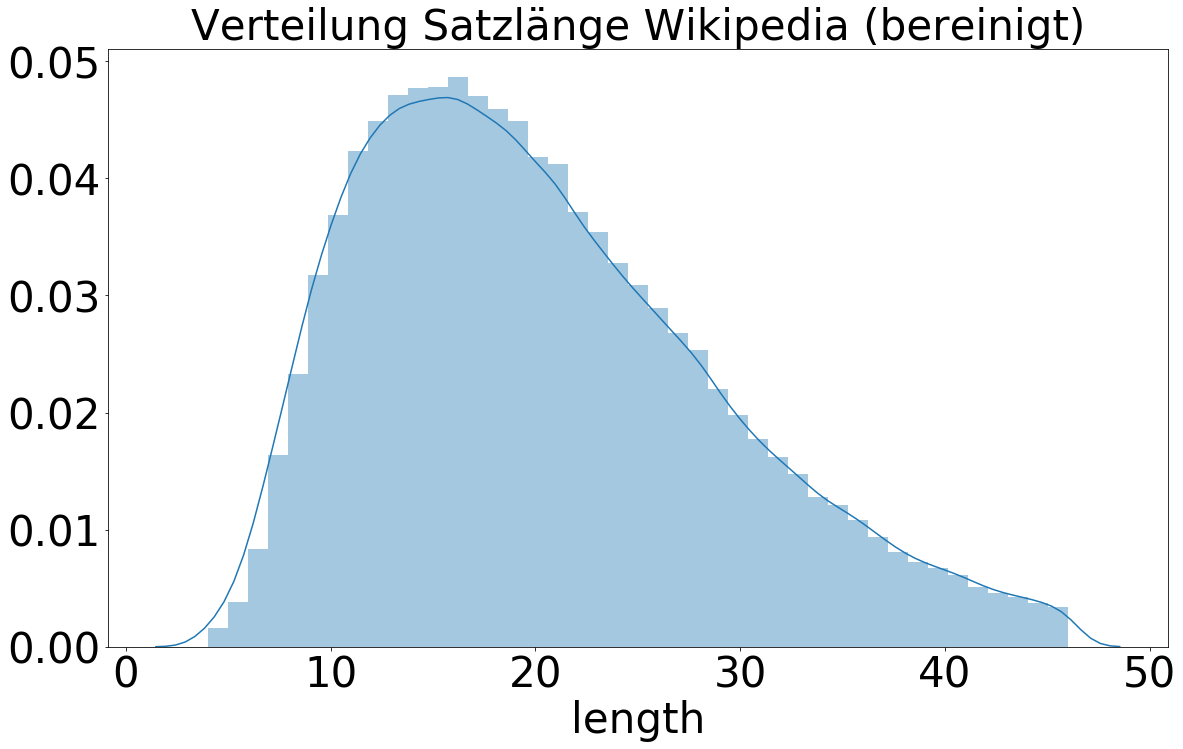
\includegraphics[width=\linewidth]{distribution_wiki_clean.png}
    \caption{Verteilung Satzlänge Wikipedia bereinigt}\label{fig:distribution_wiki_clean}
  \endminipage\hfill      
\end{figure}
\begin{table}[H]
  \centering
  \begin{tabular}{|c|c|c|c|c|c|}
    \hline
    \textbf{Datenquelle}& \textbf{25\% Quartil}& \textbf{Median}& \textbf{75\% Quartil} & \textbf{Mean} &
    \textbf{Standardabweichung}\\
    \hline
    \textbf{Klexikon}& 9 & 13 & 16 & 13.3 & 5.0\\
    \hline
    \textbf{Wikipedia}& 13 & 19 & 26 & 20.3 & 8.8\\
    \hline
  \end{tabular}
  \caption{Verteilung Anzahl Wörter Klexikon und Wikipedia ohne Ausreisser} 
\label{tab:distribution_klexi_wiki_unclean}
\end{table} 


\subsubsection{Aufbau Datensatz \flqq Ausgeglichen\frqq}
\label{sub:datensatz_ausgeglichen}
Als nächstes wurden die Grösse,  die Anzahl an Sätzen, der beide Datenquelle aneinander angepasst. Der Wikipedia
Datensatz beinhaltet ca. die doppelte Anzahl an Sätzen. Daher wurde jeder zweite Satz aus dem Wikipedia Datensatz
entfernt. Der so neu entstandene Datensatz wird wikishort genannt. In den Abbildungen
\ref{fig:article_count_ds_incl_wiki_short}, \ref{fig:sentence_count_ds_incl_wiki_short} und
\ref{fig:word_count_ds_incl_wiki_short} wird die neue Grösse der Datensätze abgebildet.
\begin{figure}[H]
  \minipage{0.32\textwidth}
    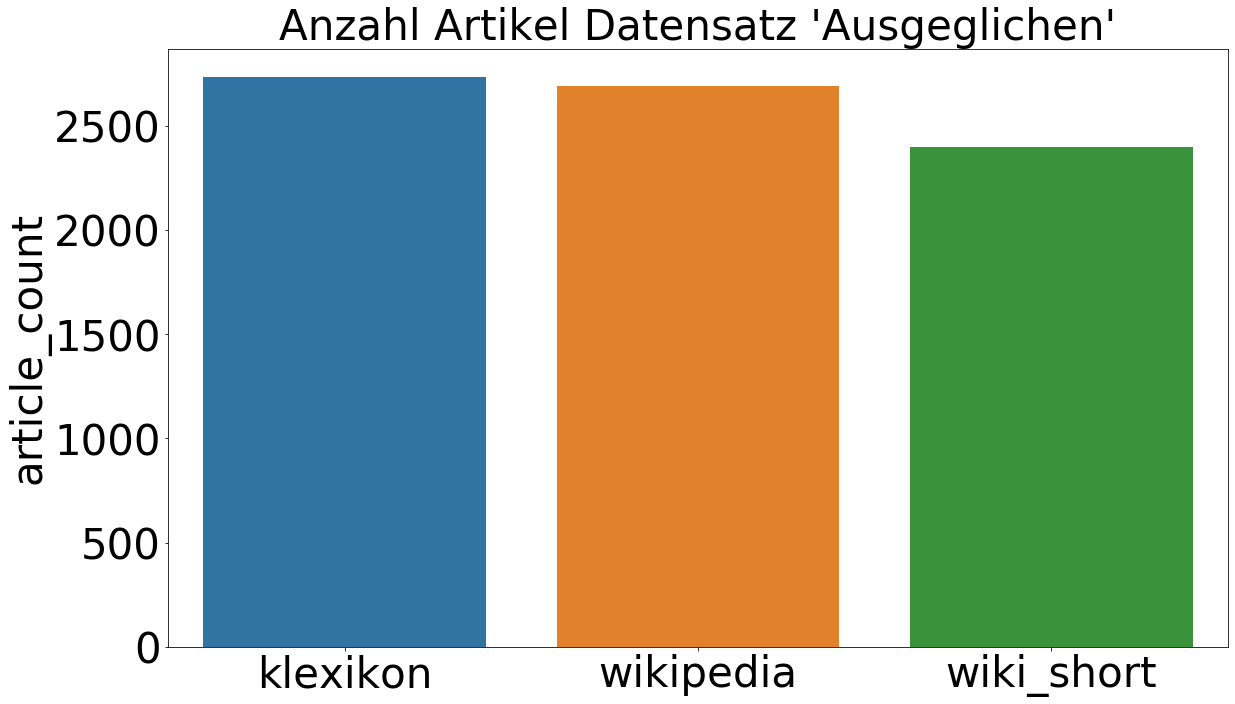
\includegraphics[width=\linewidth]{article_count_incl_wiki_short.png}
    \caption{Anz. Artikel im bereinigten Datensatz}\label{fig:article_count_ds_incl_wiki_short}
  \endminipage\hfill
  \minipage{0.32\textwidth}
    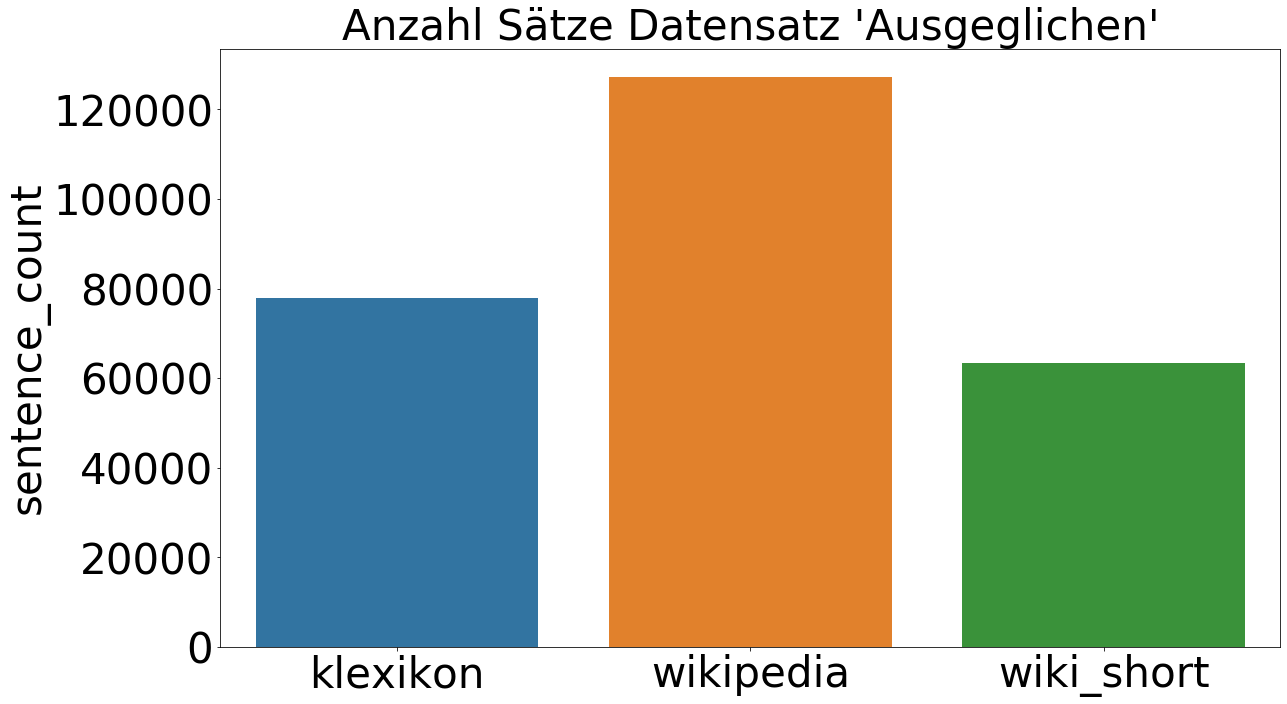
\includegraphics[width=\linewidth]{sentence_count_incl_wiki_short.png}
    \caption{Anz. Sätze im bereinigten Datensatz}\label{fig:sentence_count_ds_incl_wiki_short}
  \endminipage\hfill
  \minipage{0.32\textwidth}
    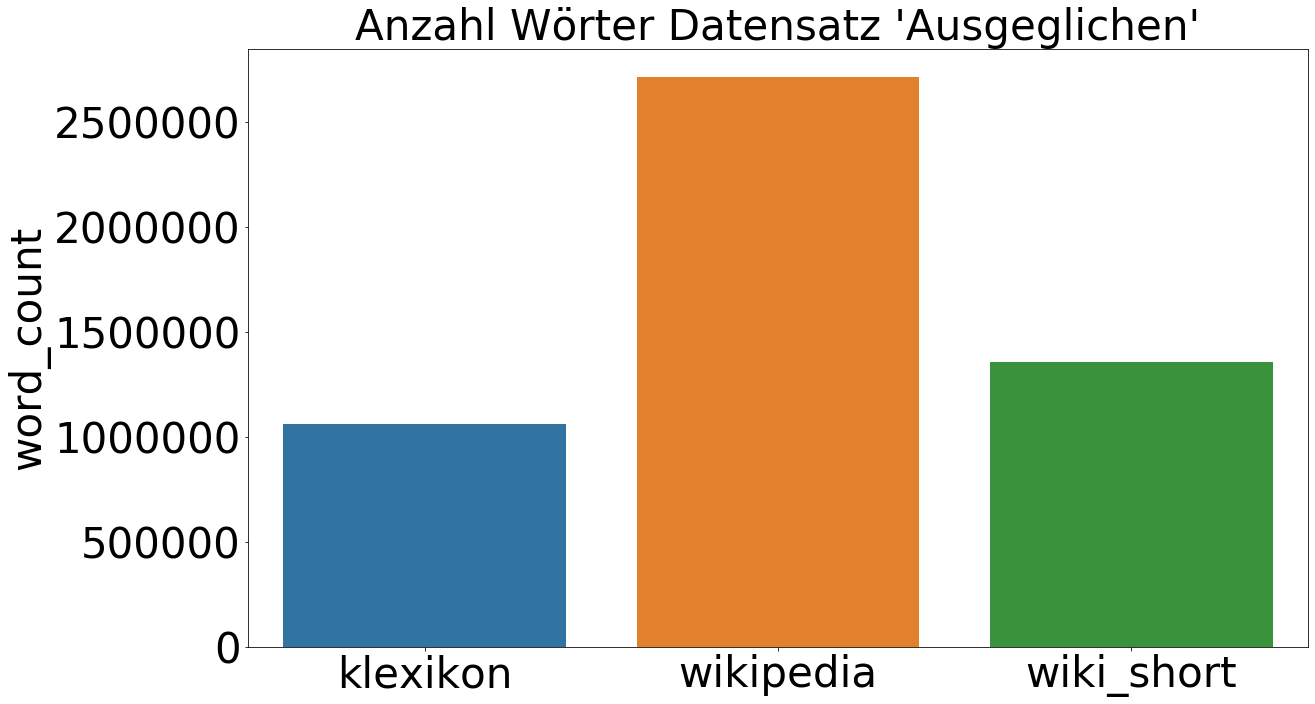
\includegraphics[width=\linewidth]{word_count_incl_wiki_short.png}
    \caption{Anz. Wörter im bereinigten Datensatz}\label{fig:word_count_ds_incl_wiki_short}
  \endminipage      
\end{figure}
\begin{table}[H]
  \centering
  \begin{tabular}{|c|c|c|c|}
      \hline
      \textbf{Datenquelle}& \textbf{Anz. Artikel}& \textbf{Anz. Sätze}& \textbf{Anz. Wörter}\\
      \hline
      \textbf{Klexikon}& 2'733 & 77'924 & 1'058'623\\
      \hline
      \textbf{Wikipedia}& 2'398 & 61'543 & 1'249'414\\
      \hline
  \end{tabular}
  \caption{Anzahl Sätze, Sätze und Wörter Klexikon, Wikipedia und Wikipedia \flqq Ausgeglichen\frqq}  
\label{tab:count_klexi_wiki_short}
\end{table}

\noindent
Da die Anzahl an Sätzen für beide Datenquellen ausgeglichen wurden, erhält dieser Datensatz die Bezeichnung \flqq
Ausgeglichen\frqq. Dies, da die Anzahl der Sätze für beide Datenquellen ausgeglichen wurden. Dabei bleibt die Verteilung
der Satzlänge auf beiden Datenquellen gleich, welches wie im Kapitel \ref{sec:abschliessende_problemdefinition}
beschrieben die Charakteristik der beiden Stile, $ erwachsen $ und $ kindlich $, beschreibt. In Abbildung
\ref{fig:distribution_both_cleaned_and_equalized} sind die beiden Verteilungen der Datenquellen noch einmal übereinander
aufgezeigt.
\begin{figure}[H]
	\centering
	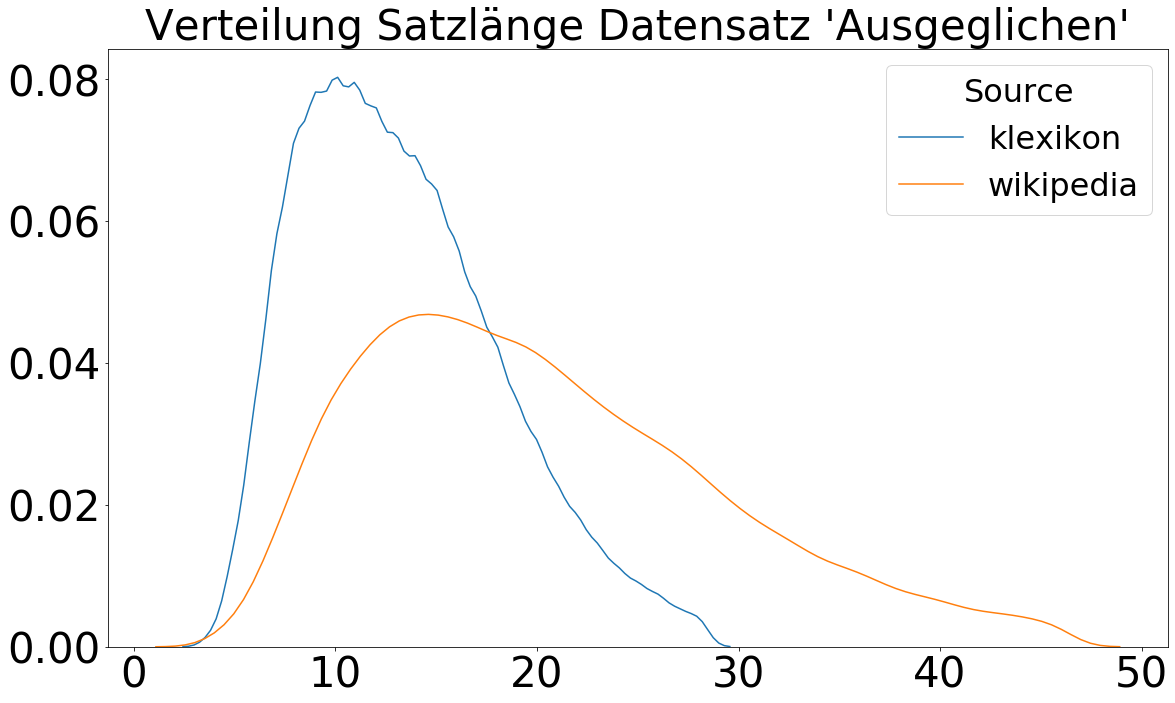
\includegraphics[scale=0.3]{distribution_both_cleaned_and_equalized.png}
	\caption{Verteilung Satzlänge Datensatz \flqq Ausgeglichen\frqq}
	\label{fig:distribution_both_cleaned_and_equalized}
\end{figure}


\subsubsection{Aufbau Datensatz \flqq Gekürzt\frqq}
\label{sub:datensatz_gekuertz}
Auf der Datenbasis des Datensatz aus \fullref{sub:statistische_analyse_des_datensatz} wurde neben dem Datensatz \flqq
Ausgeglichen\frqq, siehe \fullref{sub:datensatz_ausgeglichen}, ein zweiter Datensatz erstellt. In diesem Datensatz
sollen die beiden Stile klarer differenziert werden. Im Datensatz \flqq Ausgeglichen\frqq \ gibt es Sätze, welche sich
in der Satzlänge überschneiden. Dies soll in diesem Datensatz nicht der Fall sein. Dies bedeutet für beide Datenquellen
werden nur die Sätze verwendet die in einen gewissen Bereich fallen. Dieser Bereich soll die Stile besser definieren. Es
wurde entschieden aus der Datenquelle Klexikon nur Sätze zu verwenden, welche eine Satzlänge zwischen $ 10 $ und $ 20 $
Wörter aufweisen. Für die Datenquelle Wikipedia wurden nur Sätze, welche eine Länge zwischen $ 20 $ und $ 30 $ Wörter
enthalten. Dadurch soll ein Datensatz entstehen, in welchem die beiden Stile, welche anhand der Länge definiert werden,
klarer differenziert werden. Dieser Datensatz kann hilfreich sein, falls die Modelle die Stile aus dem Datensatz \flqq
Ausgeglichen\frqq \ nicht extrahieren kann, da die Satzlängen sich aufgrund Überschneidung zuwenig unterscheiden. Die
Verteilung der beiden Datenquelle im Datensatz \flqq Gekürzt\frqq \ sind in den Abbildungen
\ref{fig:distribution_klexi_trimmed} und \ref{fig:distribution_wiki_trimmed} zu sehen.
\begin{figure}[H]
  \minipage{0.45\textwidth}
    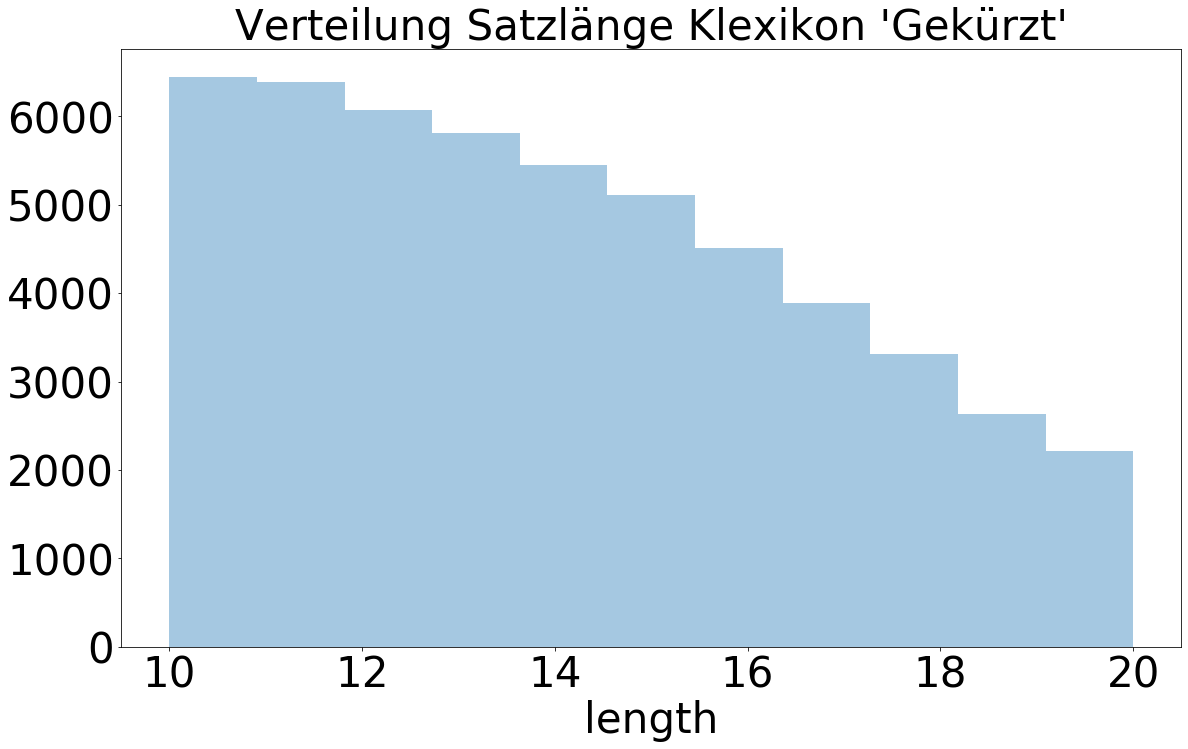
\includegraphics[width=\linewidth]{distribution_klexi_trimmed.png}
    \caption{Verteilung Satzlänge Klexikon \flqq Gekürzt\frqq}\label{fig:distribution_klexi_trimmed}
  \endminipage\hfill
  \minipage{0.45\textwidth}
    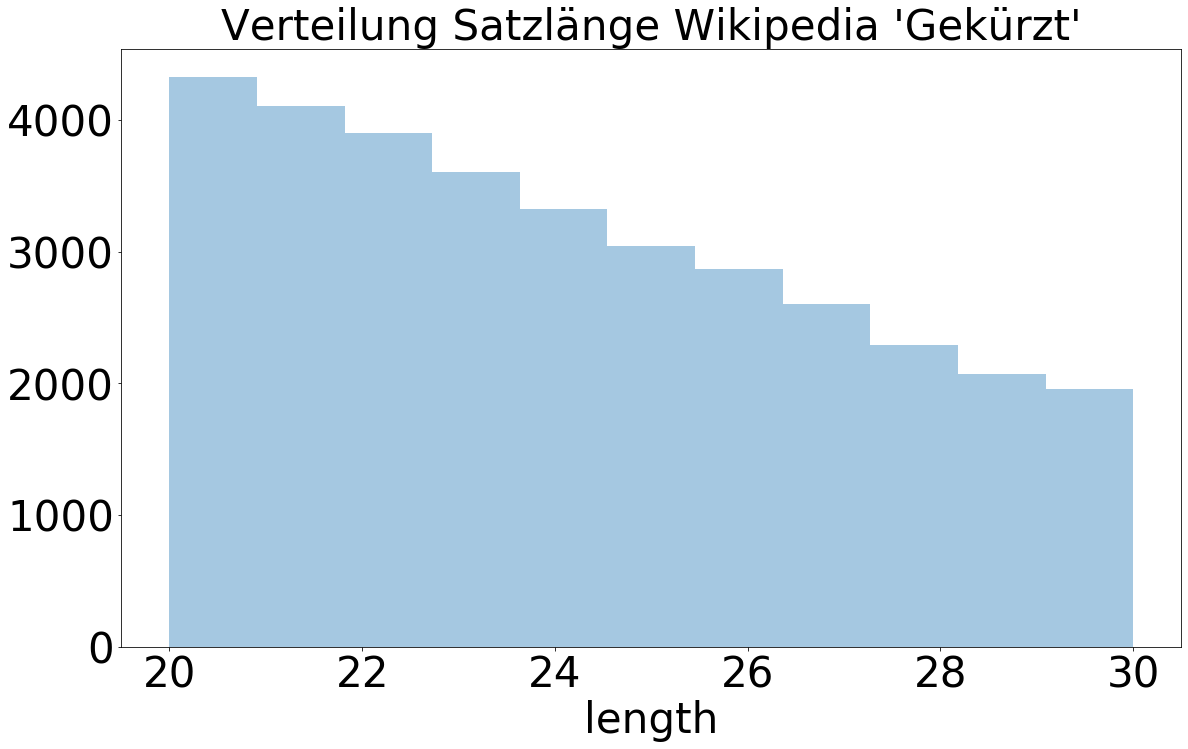
\includegraphics[width=\linewidth]{distribution_wiki_trimmed.png}
    \caption{Verteilung Satzlänge Wikipedia \flqq Gekürzt\frqq}\label{fig:distribution_wiki_trimmed}
  \endminipage\hfill
\end{figure}

\newpage

\section{Training der Modelle}
\label{sec:resultate}

Aufbauend auf den Erwähnungen in \fullref{sec:training_der_modelle} werden hier die Resultate der Modelle nach dem
Training vorgestellt. Auch sollen die Entscheidungen für die Änderungen der Hyperparameter ausgeführt werden. 
\newline
\newline
In der linken Spalte (blaue Farbe), finden sich die jeweils Resultate des Models ControlGen. In der rechten
Spalte, in Rot, sind die Resultate der CrossAlign Modelle abgebildet. Es werden drei Graphen dargestellt. Alle
Graphen zeigen die Resultate aus dem Validations Schritt des Trainings. Die erste Grafik zeigt die Genauigkeit des
durchgeführten Style Transfer. Die zweite zeigt den Verlauf der Entwicklung des \gls{BLEU} Scores für die generierten
Sätze. In der dritten Grafik wird die Verlustfunktion über die Trainingszeit dargestellt. Zum Schluss jedes Trainings
wird ein Fazit aus den Hyperparameter Einstellungen gezogen. Die Gestaltung des nächsten Trainingsdurchlauf wurde
aufgrund der Resultate der Trainings durchgeführt.

\subsection{Standard Hyperparameter}
\label{sub:standard_hyperparameter}

Zuerst wurden die beiden Modelle ControlGen und CrossAlign mit den vorgeschlagenen Hyperparameter trainiert.
Auch wurden beide Modelle auf beiden Datensätzen \flqq Ausgeglichen\frqq \ und \flqq Gekürzt\frqq \ trainiert. Die
Hyperparameter für die entsprechenden Modelle und Graphen sind in Tabelle \fullref{tab:training_standard_hyperparameter}
aufgelistet und sind im Abschnitt \ref{sub:modelle} beschrieben.
\begin{table}[ht]
	\centering
	\begin{tabular}{|l|l|l|l|l|}
    \hline
    \textbf{Hyperparameter} &
    \multicolumn{4}{c|}{\textbf{Werte}} \\
    \hline
    network & CrossAlign & CrossAlign & ControlGen & ControlGen \\
    \hline
    dataset & trimmed & equalized & trimmed & equalized \\
    \hline
    max epochs & 200 & 200 & 200 & 200 \\
    \hline
    pretrain epochs & 100 & 100 & 100 & 100 \\
    \hline
    batch size & 64 & 64 & 64 & 64 \\
    \hline
    learning rate & 0.0005 & 0.0005 & 0.0005 & 0.0005 \\
    \hline
    max len. sentences & 50 & 50 & 50 & 50 \\
    \hline
    dropout rate & 0.5 & 0.5 & 0.5 & 0.5 \\
    \hline
    number of layers & 1 & 1 & 1 & 1 \\
    \hline
    loss rec weight & 1 & 1 & 1 & 1 \\
    \hline
    trim padding & false & false & false & false \\
    \hline
    word min. occur & 3 & 3 & 3 & 3 \\
    \hline
    word embedding & embed. layer & embed.layer & embed. layer & embed. layer \\
    \hline
    dimension embedding & 100 & 100 & 100 & 100 \\
    \hline
    dimension y & 200 & 200 & 200 & 200 \\
    \hline
    dimension z & 500 & 500 & 500 & 500 \\
    \hline
    $\rho$ (rho) & 1 & 1 & 1 & 1 \\
    \hline
    $\gamma$ (gamma) & 0.1 & 0.1 & 0.1 & 0.1 \\
    \hline
    filter sizes & 1,2,3,4,5 & 1,2,3,4,5 & 1,2,3,4,5 & 1,2,3,4,5 \\
    \hline
    number of filters & 128 & 128 & 128 & 128 \\
    \hline
    \end{tabular}
	\caption{Training der Modelle mit standard Hyperparameter}
	\label{tab:training_standard_hyperparameter}
\end{table}

\subsubsection{Datensatz \flqq Ausgeglichen\frqq}

\begin{figure}[H]
  \minipage{0.45\textwidth}
    \includegraphics[width=\linewidth]{control_gen_equalized_default_full/valid_acc}
    \caption{Genauigkeit Transfer ControlGen Default \flqq Ausgeglichen\frqq}\label{fig:control_gen_equalized_default_full_valid_acc}
  \endminipage\hfill
  \minipage{0.45\textwidth}
    \includegraphics[width=\linewidth]{cross_align_equalized_default_full/valid_acc}
    \caption{Genauigkeit Transfer CrossAlign Default \flqq Ausgeglichen\frqq}\label{fig:cross_align_equalized_default_full_valid_acc}
  \endminipage\hfill   
\end{figure}

\begin{figure}[H]
  \minipage{0.45\textwidth}
    \includegraphics[width=\linewidth]{control_gen_equalized_default_full/valid_bleu}
    \caption{BLEU Score ControlGen Default \flqq Ausgeglichen\frqq}\label{fig:control_gen_equalized_default_full_valid_bleu}
  \endminipage\hfill
  \minipage{0.45\textwidth}
    \includegraphics[width=\linewidth]{cross_align_equalized_default_full/valid_bleu}
    \caption{BLEU Score Transfer CrossAlign Default \flqq Ausgeglichen\frqq}\label{fig:cross_align_equalized_default_full_valid_bleu}
  \endminipage\hfill   
\end{figure}

\begin{figure}[H]
  \minipage{0.45\textwidth}
    \includegraphics[width=\linewidth]{control_gen_equalized_default_full/valid_loss}
    \caption{Verlustfunktion ControlGen Default \flqq Ausgeglichen\frqq}\label{fig:control_gen_equalized_default_full_valid_loss}
  \endminipage\hfill
  \minipage{0.45\textwidth}
    \includegraphics[width=\linewidth]{cross_align_equalized_default_full/valid_loss}
    \caption{Verlustfunktion CrossAlign Default \flqq Ausgeglichen\frqq}\label{fig:cross_align_equalized_default_full_valid_loss}
  \endminipage\hfill   
\end{figure}
\noindent

\subsubsection{Datensatz \flqq Gekürzt\frqq}

\begin{figure}[H]
  \minipage{0.45\textwidth}
    \includegraphics[width=\linewidth]{control_gen_trimmed_default_full/valid_acc}
    \caption{Genauigkeit Transfer ControlGen Default \flqq Gekürzt\frqq}\label{fig:control_gen_trimmed_default_full_valid_acc}
  \endminipage\hfill
  \minipage{0.45\textwidth}
    \includegraphics[width=\linewidth]{cross_align_trimmed_default_full/valid_acc}
    \caption{Genauigkeit Transfer CrossAlign Default \flqq Gekürzt\frqq}\label{fig:cross_align_trimmed_default_full_valid_acc}
  \endminipage\hfill   
\end{figure}

\begin{figure}[H]
  \minipage{0.45\textwidth}
    \includegraphics[width=\linewidth]{control_gen_trimmed_default_full/valid_bleu}
    \caption{BLEU Score ControlGen Default \flqq Gekürzt\frqq}\label{fig:control_gen_trimmed_default_full_valid_bleu}
  \endminipage\hfill
  \minipage{0.45\textwidth}
    \includegraphics[width=\linewidth]{cross_align_trimmed_default_full/valid_bleu}
    \caption{BLEU Score Transfer CrossAlign Default \flqq Gekürzt\frqq}\label{fig:cross_align_trimmed_default_full_valid_bleu}
  \endminipage\hfill   
\end{figure}

\begin{figure}[H]
  \minipage{0.45\textwidth}
    \includegraphics[width=\linewidth]{control_gen_trimmed_default_full/valid_loss}
    \caption{Verlustfunktion ControlGen Default \flqq Gekürzt\frqq}\label{fig:control_gen_trimmed_default_full_valid_loss}
  \endminipage\hfill
  \minipage{0.45\textwidth}
    \includegraphics[width=\linewidth]{cross_align_trimmed_default_full/valid_loss}
    \caption{Verlustfunktion CrossAlign Default \flqq Gekürzt\frqq}\label{fig:cross_align_trimmed_default_full_valid_loss}
  \endminipage\hfill   
\end{figure}

\subsubsection{Fazit der Hyperparameter Einstellungen}

Wie in Abbildung \ref{fig:cross_align_equalized_default_full_valid_acc} und
\ref{fig:cross_align_trimmed_default_full_valid_acc} ersichtlich wird kann der Style Transfer mit dem Modell
CrossAlign nicht richtig durchgeführt werden. Dies ist aufgrund der sich nicht ändernden Genauigkeit des Transfers
zu erklären. Obwohl der \gls{BLEU} Score für den Datensatz \flqq Ausgeglichen\frqq \ höher aus fällt als für den
Datensatz \flqq Gekürzt\frqq, siehe \ref{fig:control_gen_equalized_default_full_valid_bleu},
\ref{fig:cross_align_equalized_default_full_valid_bleu}, \ref{fig:control_gen_trimmed_default_full_valid_bleu},
\ref{fig:cross_align_trimmed_default_full_valid_bleu}. Aufgrund der transferierten Sätze, siehe Repository
\fullref{sub:wipro-logs}, ist ersichtlich, dass die Länge der Sätze dabei jedoch nicht ändert. Da die Satzlängen sich
nicht ändern kann auch der hohe \gls{BLEU} Score erklärt werden, siehe \fullref{sub:BLEU}. Dies bestätigt Teilweise die
Vermutung, der sich zu stark überschneidenden Sätze, siehe \fullref{sec:aufbau_datensatz}. Daher wurde nach der Sichtung
der transferierten Sätze entschieden, die weiteren Trainings nur noch auf dem Datensatz \flqq Gekürzt\frqq \
durchzuführen. 
\newline
\newline
Die Verlustfunktion, \ref{fig:control_gen_equalized_default_full_valid_loss} und
\ref{fig:cross_align_equalized_default_full_valid_loss}, setzt sich aus der Verlustfunktion für die Diskriminatoren und
Generatoren zusammen, siehe Repository \fullref{sub:gan}. In Absprache mit der Betreuungsperson wurden daher für
den nächsten Trainingsdurchlauf entschieden, eine gewichtete Funktion auszuprobieren. Dies, da der Verlust des
Transfers einen grossen Einfluss auf den gesamt Verlust hat.

\newpage

\subsection{Standard Hyperparameter mit gewichteter Verlustfunktion}
\label{sub:weighted_hyperparameter}

In diesem Trainingsdurchlauf wurde die gewichtete Verlustfunktion für den Transfer Verlust eingefügt. Die
Hyperparameter wurde auf den Standardwerten belassen, dies um einen Vergleich zum Training ohne gewichtete
Verlustfunktionen zu erhalten. Diese Einstellungen wurden nur noch auf dem Datensatz \flqq Gekürzt\frqq \ durchgeführt.
Die Hyperparameter für die entsprechenden Modelle und Graphen sind in Tabelle
\fullref{tab:training_weighted_loss_hyperparameter} aufgelistet und sind im Abschnitt \ref{sub:modelle} beschrieben.
\begin{table}[ht]
	\centering
	\begin{tabular}{|l|l|l|}
    \hline
    \textbf{Hyperparameter} &
    \multicolumn{2}{c|}{\textbf{Werte}} \\
    \hline
    network & CrossAlign & ControlGen \\
    \hline
    dataset & trimmed & trimmed \\
    \hline
    max epochs & 200 & 200 \\
    \hline
    pretrain epochs & 100 & 100 \\
    \hline
    batch size & 64 & 64 \\
    \hline
    learning rate & 0.0005 & 0.0005 \\
    \hline
    max len. sentences & 50 & 50 \\
    \hline
    dropout rate & 0.5 & 0.5 \\
    \hline
    number of layers & 1 & 1 \\
    \hline
    loss rec weight & 0.5 & 0.5 \\
    \hline
    trim padding & false & false \\
    \hline
    word min. occur & 3 & 3 \\
    \hline
    word embedding & embed. layer & embed. layer \\
    \hline
    dimension embedding & 100 & 100 \\
    \hline
    dimension y & 200 & 200 \\
    \hline
    dimension z & 500 & 500 \\
    \hline
    $\rho$ (rho) & 1 & 1 \\
    \hline
    $\gamma$ (gamma) & 0.1 & 0.1 \\
    \hline
    filter sizes & 1,2,3,4,5 & 1,2,3,4,5 \\
    \hline
    number of filters & 128 & 128 \\
    \hline
    \end{tabular}
	\caption{Training der Modelle mit gewichteter Transfer Lossfunktion Hyperparameter}
	\label{tab:training_weighted_loss_hyperparameter}
\end{table}

\begin{figure}[H]
  \minipage{0.45\textwidth}
    \includegraphics[width=\linewidth]{control_gen_trimmed_new_loss_full/valid_acc}
    \caption{Genauigkeit Transfer ControlGen Gewichtet \flqq Gekürzt\frqq}\label{fig:control_gen_trimmed_new_loss_full_valid_acc}
  \endminipage\hfill
  \minipage{0.45\textwidth}
    \includegraphics[width=\linewidth]{cross_align_trimmed_new_loss_full/valid_acc}
    \caption{Genauigkeit Transfer CrossAlign Gewichtet \flqq Gekürzt\frqq}\label{fig:cross_align_trimmed_new_loss_full_valid_acc}
  \endminipage\hfill   
\end{figure}

\begin{figure}[H]
  \minipage{0.45\textwidth}
    \includegraphics[width=\linewidth]{control_gen_trimmed_new_loss_full/valid_bleu}
    \caption{BLEU Score ControlGen Gewichtet \flqq Gekürzt\frqq}\label{fig:control_gen_trimmed_default_new_loss_valid_bleu}
  \endminipage\hfill
  \minipage{0.45\textwidth}
    \includegraphics[width=\linewidth]{cross_align_trimmed_new_loss_full/valid_bleu}
    \caption{BLEU Score Transfer CrossAlign Gewichtet \flqq Gekürzt\frqq}\label{fig:cross_align_trimmed_new_loss_full_valid_bleu}
  \endminipage\hfill   
\end{figure}

\begin{figure}[H]
  \minipage{0.45\textwidth}
    \includegraphics[width=\linewidth]{control_gen_trimmed_new_loss_full/valid_loss}
    \caption{Verlustfunktion ControlGen Gewichtet \flqq Gekürzt\frqq}\label{fig:control_gen_trimmed_new_loss_full_valid_loss}
  \endminipage\hfill
  \minipage{0.45\textwidth}
    \includegraphics[width=\linewidth]{cross_align_trimmed_new_loss_full/valid_loss}
    \caption{Verlustfunktion CrossAlign Gewichtet \flqq Gekürzt\frqq}\label{fig:cross_align_trimmed_new_loss_full_valid_loss}
  \endminipage\hfill   
\end{figure}

\subsubsection{Fazit der Hyperparameter Einstellungen}
Die Resultate des Trainings \fullref{sub:weighted_hyperparameter} sind nahezu identisch mit
\fullref{sub:standard_hyperparameter}. Daraus kann die Verbesserung der Modelle mit einer Gewichtung des Transfer
Verlust nicht erreicht werden. Weiter wurde nach diesem Trainingsdurchlauf entschieden, weitere Trainings nur noch auf
dem ControlGen Modell durchzuführen. Dies ist aufgrund der sich nicht ändernden Genauigkeit des Transfers. In
\ref{fig:control_gen_trimmed_new_loss_full_valid_acc} und \ref{fig:cross_align_trimmed_new_loss_full_valid_acc} ist
ersichtlich dass, das Modell CrossAlign den Style Transfer nicht wie gewünscht durchführt. 

\newpage

\subsection{ControlGen mit grösseren Dimensionen}
\label{sub:bigger_embedding_hyperparameter}

Da der \gls{BLEU} Score für die ControlGen Modelle niedrig ausfällt, wurde entschieden, die Dimension für das Word
Embedding, sowie den Kontext und Style Raum zu vergrössern. Dadurch hat das Modell mehr Variablen für das Training zur
Verfügung. Damit das Modell trainiert werden kann ist mehr \gls{RAM} auf der Grafikkarte nötig. Daher wurde für dieses
Training eine Grafikkarte mit 32GB \gls{RAM}, NVIDIA Tesla 100V, verwendet. Die Hyperparameter für die entsprechenden
Modelle und Graphen sind in Tabelle \fullref{tab:training_big_embedding_hyperparameter} aufgelistet und sind im
Abschnitt \ref{sub:modelle} beschrieben.
\begin{table}[ht]
	\centering
	\begin{tabular}{|l|l|}
    \hline
    \textbf{Hyperparameter} &
    \textbf{Werte} \\
    \hline
    network  & ControlGen \\
    \hline
    dataset  & trimmed \\
    \hline
    max epochs & 200 \\
    \hline
    pretrain epochs & 100 \\
    \hline
    batch size & 64 \\
    \hline
    learning rate & 0.0005 \\
    \hline
    max len. sentences & 50 \\
    \hline
    dropout rate & 0.5 \\
    \hline
    number of layers & 1 \\
    \hline
    loss rec weight & 1 \\
    \hline
    trim padding & false \\
    \hline
    word min. occur & 3 \\
    \hline
    word embedding & embed. layer \\
    \hline
    dimension embedding & 300 \\
    \hline
    dimension y & 300 \\
    \hline
    dimension z & 900 \\
    \hline
    $\rho$ (rho) & 1 \\
    \hline
    $\gamma$ (gamma) & 0.1 \\
    \hline
    filter sizes & 1,2,3,4,5 \\
    \hline
    number of filters & 128 \\
    \hline
    \end{tabular}
	\caption{Training der Modelle mit grösseren Embedding Hyperparametern}
	\label{tab:training_big_embedding_hyperparameter}
\end{table}

\begin{figure}[H]
    \centering
    \includegraphics[scale=0.25]{control_gen_trimmed_bigger_embedding_full/valid_acc}
    \caption{Genauigkeit Transfer ControlGen Dimensionen \flqq Gekürzt\frqq}\label{fig:control_gen_trimmed_bigger_embedding_full_valid_acc}
\end{figure}

\begin{figure}[H]
    \centering
    \includegraphics[scale=0.25]{control_gen_trimmed_bigger_embedding_full/valid_bleu}
    \caption{BLEU Score ControlGen Dimensionen \flqq Gekürzt\frqq}\label{fig:control_gen_trimmed_bigger_embedding_full_valid_bleu}
\end{figure}

\begin{figure}[H]
    \centering
    \includegraphics[scale=0.25]{control_gen_trimmed_bigger_embedding_full/valid_loss}
    \caption{Verlustfunktion ControlGen Dimensionen \flqq Gekürzt\frqq}\label{fig:control_gen_trimmed_bigger_embedding_full_valid_loss}
\end{figure}

\subsubsection{Fazit der Hyperparameter Einstellungen}
Wie erwartet, konnte der \gls{BLEU} Score mit einem grösseren Raum verbessert werden. Dies jedoch nur in der
Trainingsphase des Vortrainings, siehe \fullref{sub:control_gen}. Die transferierten Sätze sind jedoch auch mit diesen
Trainingseinstellungen nicht zufriedenstellend. Auf eine weitere Erhöhung der Dimensionen wurde aufgrund von Zeit- und
Ressourcenmangel verzichtet. Zu diesem Zeitpunkt im Projekt wurde entschieden auf weitere Trainings zu verzichten. Es
scheint so, dass mit dem verwendeten Modellen kein zufriedenstellendes Resultat erreichen werden kann. Begründungen für
diese Annahme werden in \fullref{ch:Eval} aufgeführt.

\section{Prototyp}
\label{sec:prototyp}
Um die einzelnen Modelle auch mit einem beliebigen Eingabesatz zu testen wurde ein Prototyp in Python (\cite{python})
entwickelt, welcher ein gewisses Modell laden kann und anschliessend einen eingegebenen Satz in einen anderen
transferiert.
\newline
\newline
Der Prototyp wurde aus zeitlichen Gründen ohne User Interface entwickelt und ist daher ein Python Skript mit einem
Command Line Interface. Die Umsetzung wurde bewusst sehr minimal gehalten, da der Fokus dieser Arbeit mehrheitlich auf
dem Erarbeiten vielversprechender Modelle war anstatt auf der Entwicklung eines erweiterten Prototypen. Dies wurde
aufgrund der dürftigen Ergebnisse der trainierten Modelle entschieden.
\newline
\newline
Um die Benutzung und Installation des Prototypen zu erleichtern wurde ein Docker Image (\cite{docker}) geschrieben,
welches als erstes Git herunterlädt, um das \fullref{sub:wipro-source} Git klonen zu können. Anschliessend werden die
PIP Requirements des Projektes installiert so dass alles korrekt funktioniert. Bei jedem ausführen des Containers wird
der Prototyp direkt ausgeführt, so dass dieser benutzt werden kann ohne weitere Schritte. Das Docker Image wurde auf
Docker Hub (\cite{docker_hub}) geladen, so dass dieses wie ein Git Repository, heruntergeladen werden kann. Dieses Image
ist unter der URL \hyperlink{https://hub.docker.com/repository/docker/fabiangroeger96/wipro-prototype}{Docker Image
Prototype} erreichbar und ist öffentlich. Das Dockerfile um das Docker Image zu erstellen befindet sich im
\fullref{sub:wipro-source} Projekt.
\newline
\newline
Wenn das Docker Image ausgeführt wird, startet sogleich der Prototyp. Als Erstes wird nach dem Modell, welches für den
Style Transfer gebraucht wird, gefragt. Dabei stehen drei verschiedene zur Verfügung:
\begin{enumerate}
  \setlength\itemsep{0em}
  \item \textbf{cross-align-trimmed-new-loss-full}, ein \fullref{sub:cross_align} Netzwerk trainiert auf dem \flqq
  wipro-trimmed\frqq \ Datensatz über 200 Epochen mit den default Hyperparametern, \fullref{sub:standard_hyperparameter}
  \item \textbf{control-gen-trimmed-bigger-embedding-full}, ein \fullref{sub:control_gen} Netzwerk trainiert auf dem \flqq
  wipro-trimmed\frqq \ Datensatz über 200 Epochen mit den Hyperparametern für ein grösseres Embedding,
  \fullref{sub:bigger_embedding_hyperparameter}
  \item \textbf{control-gen-equalized-default-full}, ein \fullref{sub:control_gen} trainiert auf dem \flqq
  wipro-trimmed\frqq \ Datensatz über 200 Epochen mit den default Hyperparametern, \fullref{sub:standard_hyperparameter}
\end{enumerate}
\noindent
Nach dem Eingeben der Nummer des gewünschten Modells wird das Modell initialisiert und anschliessend die gespeicherten
Gewichte geladen, dieser Prozess kann je nach Computer etwas länger dauern. Als Nächstes kann ein Satz zum Transfer
eingegeben werden. Dieser wird anschliessend zu einem Batch hinzugefügt und dem Modell übergeben. Der eine Output ist
danach der transferierte Satz, welcher noch aus einem encodierten Vektor der Wörter besteht. Diesen kann man anhand des
Vokabulars des Modells in Wörter zurückmappen. Als zweiter Output ist der rekonstruierte Satz, welcher auch mittels dem
Vokabular zurück transferiert wird. Diese beiden Sätze werden anschliessend ausgegeben und dargestellt.

\begin{figure}[H]
  \centering
  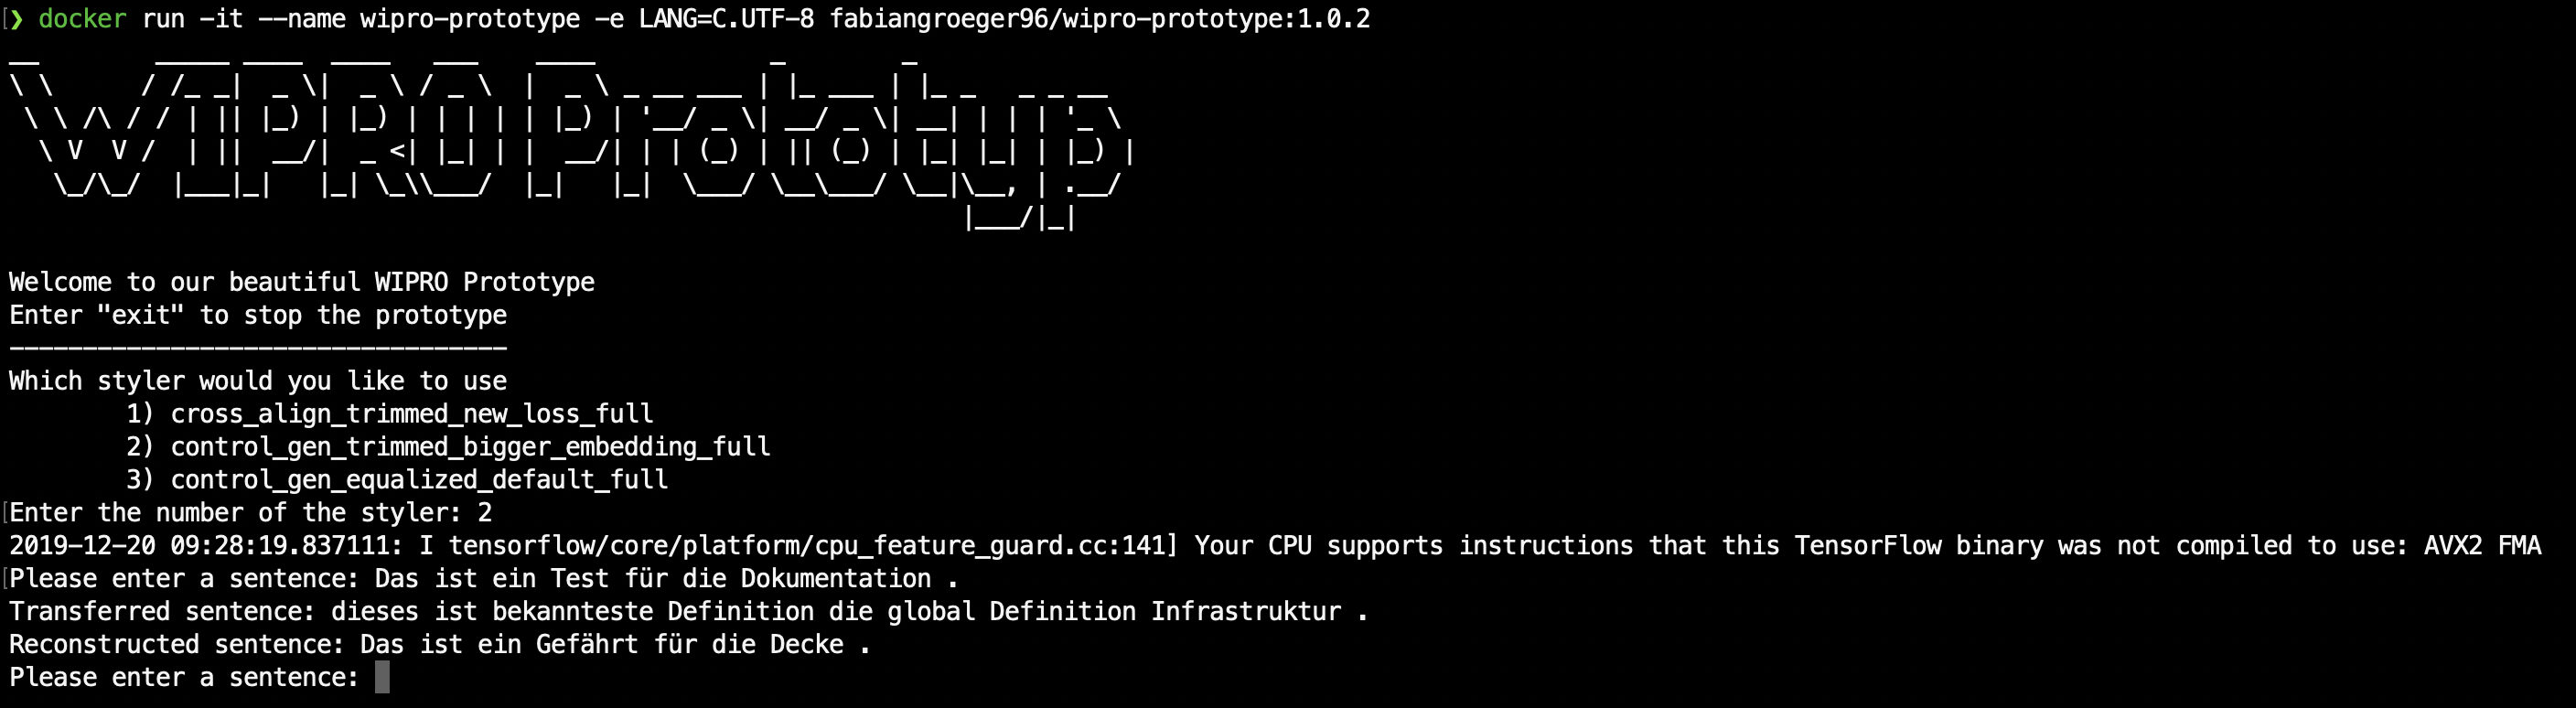
\includegraphics[scale=0.275]{prototyp}
  \caption{Command Line Interface des Prototypen}\label{fig:prototyp}
\end{figure}
